\documentclass[conference]{IEEEtran}
\usepackage[T1]{fontenc}
\usepackage{microtype}
\usepackage{amsmath}
\usepackage{booktabs}
\usepackage{graphicx}
\usepackage{xcolor}
\usepackage{tikz}
\usetikzlibrary{arrows.meta,positioning,calc}
\usepackage{balance}
\usepackage{stfloats}
\usepackage[hidelinks]{hyperref}
\hypersetup{pdftitle={KVFold: Expanding Cache Capacity for LLM Agents with Lossless Compression},
            pdfsubject={ICDE demonstration paper}}
\definecolor{fpInk}{HTML}{172634}
\definecolor{fpBlue}{HTML}{1D62D0}
\definecolor{fpTeal}{HTML}{007E6A}
\definecolor{fpOrange}{HTML}{D96C05}
\definecolor{fpPurple}{HTML}{735892}
\tikzset{
  fpbox/.style={draw,rounded corners=2pt,align=center,inner sep=5pt,
                minimum height=0.73cm,line width=0.65pt},
  fparrow/.style={-{Stealth[length=1.7mm]},line width=0.8pt,draw=fpInk},
  fpboth/.style={{Stealth[length=1.7mm]}-{Stealth[length=1.7mm]},
                 line width=0.8pt,draw=fpInk}
}
\title{KVFold: Expanding Cache Capacity for \mbox{LLM Agents} with Lossless Compression}
\author{\IEEEauthorblockN{Working draft}
\IEEEauthorblockA{Author information to be supplied}}
\flushbottom
% Consistent space around floats; keep the IEEE text size and margins.
\setlength{\textfloatsep}{8pt plus 2pt minus 2pt}
\setlength{\dbltextfloatsep}{8pt plus 2pt minus 2pt}
\setlength{\intextsep}{8pt}
\begin{document}
\bstctlcite{kvfoldBibControl}
\maketitle

\begin{abstract}
Large language model (LLM) agents often reuse long prompt prefixes when continuing tasks or resuming
sessions. Caching the corresponding key/value (KV) states avoids repeated
prefill, but limited cache capacity constrains request concurrency and history
retention. We present KVFold, a lossless KV-cache compression system that uses
high-byte coding to expand GPU and external-cache capacity while preserving
the original bfloat16 (BF16) bits. Pool mode stores compressed KV on the GPU and
reconstructs values for attention. Tier mode compresses KV in LMCache while
retaining the native GPU cache layout and attention implementation. In
experiments replaying coding-agent session traces with a fixed 54~GiB KV
budget per GPU, pool mode increases usable capacity from 1.18M to 1.59M
tokens. We demonstrate KVFold through an interactive coding session and
recorded trace replays from the InferenceX AgentX benchmark: users inspect
prefix reuse, GPU capacity, and history retention, and compare raw and
compressed runs under fixed cache budgets.
\end{abstract}

\section{Introduction}
% [PDF 批注 1 | 2026-11-11]
% 位置：原 fragpack_demo(16).pdf 第 1 页，Introduction 首段。
% 原始意见：这个背景太奇怪了。一般直接就讲KV Cache的重要性了。不需要这么一个场景。
% 处理：已删除开场场景，直接说明 KV Cache 对生成和跨请求前缀复用的作用。
% [PDF 批注 2 | 2026-11-11]
% 位置：原 fragpack_demo(16).pdf 第 1 页，Introduction 第二段。
% 原始意见：这一段不知道想表达什么，有告诉AI这一段要表达什么么？
% 处理：已明确本段主旨；GPU 容量限制活跃请求，外部缓存容量限制历史保留，
% 二者共同引出降低每个 token 的 KV 存储开销这一动机。
% [PDF 批注 3 | 2026-11-11]
% 位置：原 fragpack_demo(16).pdf 第 1 页，Introduction 中首次介绍 pool mode 处。
% 原始意见：衔接太不自然了。还没讲清楚KVFold的定位就直接讲KVFold的两个模式了。KVFold的介绍应该是下一段的。
% 处理：已先交代压缩动机与无损目标，下一段独立介绍 KVFold 的系统定位，
% 再另起一段概述两种模式；具体字节编码细节保留在 System Description。
Key/value (KV) caching avoids repeated computation by reusing attention states
during generation and across requests with shared prefixes. This reuse is
particularly useful for large language model (LLM) agents, whose successive
calls often share long
contexts. Retaining these states, however, requires substantial memory. For
Qwen3-30B-A3B, each token requires 96~KiB of bfloat16 (BF16) KV across all layers, or
48~KiB per rank with a tensor-parallel (TP) degree of two. GPU capacity
therefore limits active contexts, while external cache capacity limits how
much history can be retained for later reuse.

To make better use of this capacity, vLLM's PagedAttention~\cite{vllm}
organizes KV into fixed-size blocks allocated on demand in noncontiguous GPU
memory. This reduces fragmentation and allows requests with common prefixes to
share physical blocks. SGLang's RadixAttention~\cite{sglang} uses a radix
tree to reuse cached prefixes across requests. LMCache~\cite{lmcache} extends reuse beyond GPU memory
by storing KV in host memory or storage and retrieving it for later requests.
Other methods reduce the retained token set: H$_2$O~\cite{h2o} keeps
recent and high-attention tokens, while StreamingLLM~\cite{streamingllm}
retains initial attention sinks with a recent-token window.

These sharing,
offloading, and token-selection mechanisms do not by themselves reduce the
bytes per retained KV value. Reducing this cost requires a more compact
representation.
FlexGen~\cite{flexgen} combines GPU/CPU/disk offloading with low-bit
compression, and KVQuant~\cite{kvquant} tailors KV quantization to channel
distributions and outliers. KIVI~\cite{kivi} quantizes
keys per channel and values per token, using two-bit representations suited to
their different distributions. For context transfer, CacheGen~\cite{cachegen}
quantizes differences between nearby tokens and then applies arithmetic coding
to reduce the data sent when loading a context. These quantization approaches save space by
approximating KV values. CacheGen's lossless coding preserves the quantized
representation, so it does not recover the original BF16 bits.

Lossless compression can reduce storage while preserving these bits by
exploiting redundancy in the underlying representation. nvCOMP~\cite{nvcomp}
provides general-purpose GPU codecs, while SplitZip~\cite{splitzip} separates
BF16 exponents from the remaining bits and encodes frequent exponents
compactly for transfer between prefill and decode workers. Using these
representations in a paged cache also requires efficient restoration and
allocation. If decoding produces a contiguous buffer, the recovered values
must be scattered into their assigned KV pages, adding data movement and
temporary storage. External allocators must also account for encoded record
lengths so that smaller records allow more history to be retained.

To address these integration requirements, we present KVFold, a lossless
KV-cache compression system for LLM agents. KVFold combines a compact BF16
representation with paged restoration and compressed GPU execution, and
allocates external storage according to encoded sizes. Two integration paths
accommodate different GPU cache layouts:
\begin{itemize}
\item \emph{Pool mode} keeps completed KV blocks compressed on the GPU and
reconstructs them as needed for attention.
\item \emph{Tier mode} applies compression in LMCache while retaining the
native GPU cache layout and attention implementation.
\end{itemize}
Both modes use lossless high-byte coding and offline calibration, with
record layouts tailored to their access patterns.

\begin{figure*}[t]
\centering
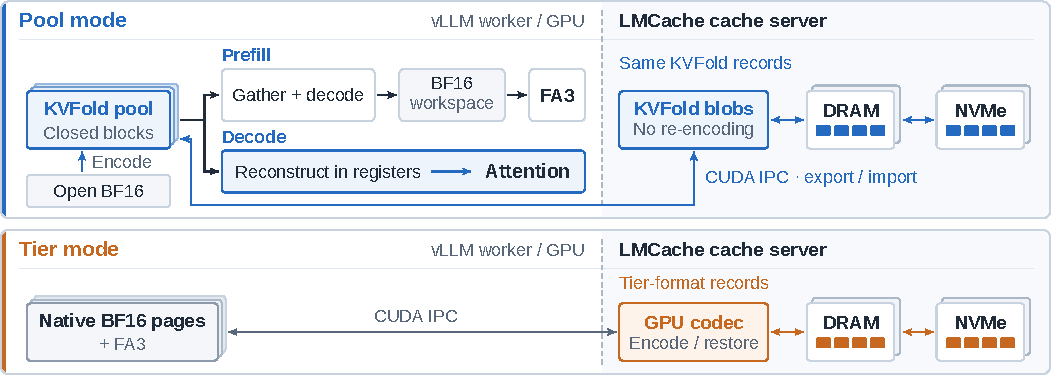
\includegraphics[width=0.90\textwidth]{images/figure1-architecture-refined.pdf}
\caption{KVFold's integration paths: pool mode exports its compressed GPU
records unchanged, whereas tier mode retains native GPU pages and applies
a cache-server codec. Dashed boundaries separate worker and cache-server
processes; LMCache manages DRAM and NVMe. FA3 denotes
FlashAttention-3~\cite{fa3neurips}.}
\label{fig:architecture}
\end{figure*}

\section{System Description}
\label{sec:design}
KVFold changes how KV is represented and recovered while leaving scheduling
and cache management to the serving stack (Fig.~\ref{fig:architecture}).
vLLM 0.30 schedules requests and allocates logical 128-token blocks, while
LMCache 0.5.6's multiprocess server handles external lookup, LRU eviction,
write-through, and prefetch. The pool backend loads through a vLLM plugin
without modifying vLLM's source.

\subsection{Compressing closed blocks in the GPU pool}
Compressing a block while it is still receiving KV would require repeated
updates. KVFold therefore keeps open blocks in BF16 staging and encodes them
after attention once they are full. The immutable records support subsequent
attention and external export without re-encoding.

Each KVFold record holds 128 tokens from one layer, one KV head,
and either the K or V tensor. The encoder retains every low byte and
replaces frequent high bytes with short codes from tables calibrated
offline for each layer, head, and K or V tensor. Three-bit codes identify
the most frequent high bytes. An escape introduces a four-bit selector
that addresses an extended table or marks a raw byte, so values outside
both tables can also be recovered exactly. Together with the retained low
bytes, these alternatives preserve every original BF16 bit, as illustrated
in Fig.~\ref{fig:record}.

\begin{figure}[!ht]
\centering
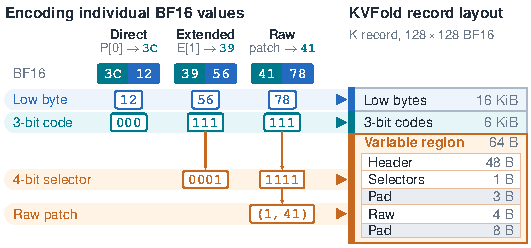
\includegraphics[width=\columnwidth]{images/figure2-record-map.pdf}
\caption{An illustrative KVFold record. P and E denote the primary and
extended high-byte tables. Low bytes are unchanged. BF16 values and bytes
are hexadecimal; codes and selectors are binary. Selectors 0001 and 1111
pack into F1, low nibble first. Raw patch (1,~41) stores zero-based escape
ordinal 1 and high byte 41. The variable region occupies 64~B
(limit: 2~KiB). Not to scale.}
\label{fig:record}
\end{figure}

Scalars are stored in the attention kernel's fragment order, so the codes
and low bytes follow the order needed to reconstruct its operands. Within each layer, a
block's K and V records share a page. With four KV heads, for example,
a page occupies 186~KiB instead of 256~KiB, allowing the same budget to
hold 1.376 times as many pages before auxiliary backend buffers are counted. Records that
exceed the encoding limit or do not fit in the shared page use uncompressed
overflow slots. Usable token capacity also depends on staging, overflow,
and attention workspace costs.

\subsection{Computing attention from compressed KV}
During \emph{prefill}, the adapter gathers a context's KV into a temporary
BF16 workspace for the current layer, decoding compressed records and copying
values from open blocks. This lets an unmodified FlashAttention-3 (FA3) kernel
process many query tokens while completed blocks remain compressed in the pool.

During \emph{decode}, each request contributes a new query token, and
materializing its full context would add a BF16 write before attention
reads the values again. KVFold instead fuses reconstruction with attention.
The kernel divides the context into page ranges, prefetches encoded records
into shared memory, and reconstructs operands in registers for tensor-core
computation. A final kernel combines the partial softmax states from those
ranges. This path avoids writing the decoded context to GPU global memory
and supports decode-only CUDA graph replay.

Although both attention paths reconstruct the original KV bits, fused
attention and FA3 can use different floating-point reduction orders. We
therefore distinguish KV byte equality from generated-text equality when
presenting the demonstration's checks.



\subsection{Storing KV in LMCache}
External caching extends the lifetime of a prefix beyond its residence on
the GPU. In pool mode, the completed blocks are already compressed, so
KVFold exports their existing records instead of decoding and encoding
them again. Each relocatable blob contains one 128-token block across all
layers, together with its dimensions, table identity, and lengths. When
the prefix is requested again, the importer restores the records and their
tables into the GPU pool. A failed validation causes the affected KV to be
recomputed.

Tier mode serves deployments that retain native GPU pages and attention.
Here, the cache server applies the codec to KV received from those pages.
The tier codec shares pool mode's offline per-layer, per-head K/V
calibration, but uses token-order records and a different escape encoding to suit page
restoration. Grouped indices locate the escape streams needed for a tile,
so the decoder can recover that tile without scanning all preceding tiles.
The codec's tables are fixed at startup and identified by a digest. If an encoded
chunk would be larger than its raw form, the server stores it uncompressed.

Tier mode integrates encoding and recovery into the existing transfer
operations. After the corresponding model step completes, the server encodes
full chunks into
fixed-capacity GPU codec slots, and a background worker commits them to
DRAM. When loading a compressed chunk, the decoder writes directly into
destination pages if the chunk can be restored in full. Raw records and
partially shared leading chunks use scratch space before scattering into their
assigned pages. CUDA events order transfer, decoding, and page reuse on
this load path without host waits.

Because smaller records expand capacity only if allocations shrink accordingly,
LMCache uses encoded lengths for storage and prefetch. Each TP rank stores its
own objects, with 4~KiB alignment for NVMe I/O.

\section{Demonstration Plan}
\label{sec:demo}
To show how compression affects reuse and latency, the console
(Fig.~\ref{fig:views}) offers a live prefix-reuse view and recorded GPU-capacity
and history-retention views, each identifying its model, mode, and cache configuration.

The live prefix-reuse view runs Qwen3-4B in pool mode on one H800 PCIe GPU, with
BF16 weights and KV; the capacity and retention views display recorded
results from Claude Code session traces replayed with SemiAnalysis's
InferenceX AgentX benchmark~\cite{agentx}, using Qwen3-30B-A3B with FP8
weights and BF16 KV on two H800 SXM GPUs (TP~2).
In these recorded runs, $P$ denotes the number of live root sessions, and $S$
is the maximum number of concurrent requests.
A planned eight-minute walkthrough covers Build/Append/Edit early/Restore,
then $S=8$ or $12$, and finally 640~GiB or 2~TiB of NVMe capacity.
The console reports cached-token counts, KV sizes, and time to first token
(TTFT) for the live interaction, plus waiting requests and latency for the
selected recorded runs.

\begin{figure*}[!t]
\centering
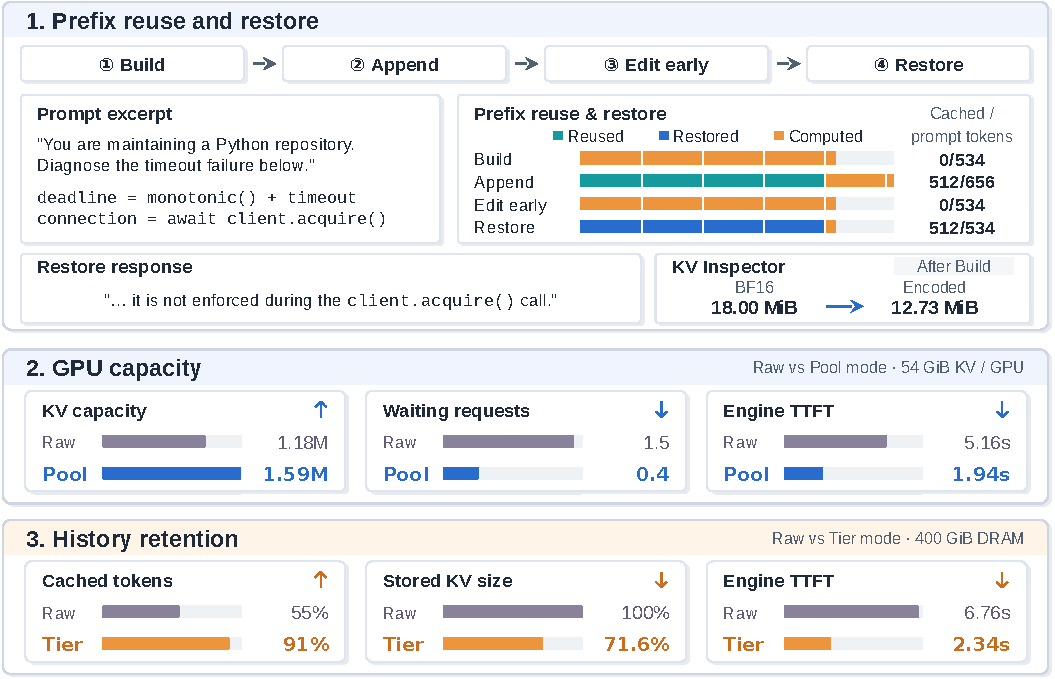
\includegraphics[width=\textwidth]{images/fig3_b_units.pdf}
\caption{Recomposed console views with selected elements.
(1) Saved Qwen3-4B interaction:
the four operations reveal reused, restored, and newly computed tokens.
The Inspector shows BF16 and encoded sizes after Build. (2, 3) Qwen3-30B-A3B capacity
comparisons on coding-agent traces from InferenceX AgentX:
$P=64$, 400~GiB DRAM; (2) $S=12$, 2~TiB NVMe; (3) $S=8$, 640~GiB NVMe.
Within each metric, paired bars use the same zero-based scale. KV capacity is in tokens; waiting
requests and TTFT are means, with TTFT in seconds. Cached tokens include
GPU and external hits; stored bytes are normalized to the raw size.}
\label{fig:views}
\end{figure*}

% Keep both result tables in one float so their columns remain aligned.
\begin{table*}[!b]
% Source: main(11).pdf, p.10, Table V; printed values retained verbatim.
\begin{minipage}[t]{\columnwidth}
\centering
\caption{GPU capacity: 54 GiB KV/GPU, $P=64$, 400 GiB DRAM, 2 TiB NVMe.
Waiting is the mean vLLM queue length; TTFT is mean engine TTFT.}
\label{tab:gpu}
\small
\setlength{\tabcolsep}{3pt}
\begin{tabular*}{\columnwidth}{@{\extracolsep{\fill}}rlrrrr@{}}
\toprule
$S$ & Mode & KV tokens & Waiting &
\begin{tabular}[t]{@{}r@{}}TTFT\\(s)\end{tabular} &
\begin{tabular}[t]{@{}r@{}}Goodput\\(req/min)\end{tabular} \\
\midrule
8  & Raw  & 1.18M & 0.3 & 1.69 & 15.1 \\
8  & Pool & 1.59M & 0.2 & 1.34 & 16.2 \\
12 & Raw  & 1.18M & 1.5 & 5.16 & 10.6 \\
12 & Pool & 1.59M & 0.4 & 1.94 & 14.9 \\
\bottomrule
\end{tabular*}
\end{minipage}\hfill
% Source: main(11).pdf, p.9, Table III; same P/S and metric definitions.
\begin{minipage}[t]{\columnwidth}
\centering
\caption{History retention: $P=64$, $S=8$, 400 GiB DRAM. Cached is the
GPU/external prompt-token hit share; TTFT is mean engine TTFT.}
\label{tab:tiers}
\small
\setlength{\tabcolsep}{3pt}
\begin{tabular*}{\columnwidth}{@{\extracolsep{\fill}}llrrr@{}}
\toprule
NVMe & Mode & Cached &
\begin{tabular}[t]{@{}r@{}}TTFT\\(s)\end{tabular} &
\begin{tabular}[t]{@{}r@{}}Goodput\\(req/min)\end{tabular} \\
\midrule
640 GiB & Raw  & 0.55 & 6.76 & 4.6 \\
640 GiB & Tier & 0.91 & 2.34 & 13.5 \\
2 TiB   & Raw  & 0.94 & 1.69 & 15.1 \\
2 TiB   & Tier & 0.94 & 1.85 & 15.4 \\
\bottomrule
\end{tabular*}
\end{minipage}
\end{table*}

% Keep the scenario heading and its opening paragraph together.
\begin{samepage}
\subsection*{Scenario 1: extend a task and inspect prefix reuse}
Users begin with \emph{Build}, submitting repository context and a bug
report asking the model to ``Diagnose the timeout failure.'' They then
extend the task through \emph{Append}, adding ``Write a regression test.''
The prefix strip distinguishes reused from newly computed tokens alongside
cached-token counts, TTFT, and the response.\par
\end{samepage}

Editing an earlier token through \emph{Edit early} limits reuse to complete
128-token blocks preceding
that change. To revisit the original request, users choose \emph{Restore}.
The console waits for external saves, resets the GPU prefix cache, and
replays the original prompt. In the saved session, this restored 512 tokens
from LMCache DRAM.

After Build, the KV Inspector checks export/import integrity by comparing
the decoded KV values before and after transferring an encoded block
through host memory into an independent GPU scratch store. It displays sizes, checksums,
and mismatch counts, with byte-for-byte agreement across all layers of the
captured 128-token block in the saved run. Separate CPU samples exercise
escapes and raw fallback, while an earlier output check found identical
greedy outputs for 192 repeat-trace requests in raw and tier modes under
matching native attention paths.

Beyond the console, a recorded microbenchmark compared restoration paths on one H800 SXM,
using 3~GiB of Qwen3-30B-A3B KV in 256-chunk calls.
SplitZip reached 1,264~GB/s when
decoding into its buffer, but 376~GB/s including scatter into paged KV.
An earlier KVFold prototype restored directly into pages at 1,229~GB/s.
Their compressed-to-raw ratios were 0.768 and 0.716, respectively.
All restores were byte-exact, and throughput counts original bytes.

\subsection*{Scenario 2: explore GPU capacity limits}
Users select $S=8$ or $S=12$ in the GPU-capacity view to compare recorded
raw and pool runs under a 54~GiB GPU KV budget (Table~\ref{tab:gpu}).
Because the external tiers retain the working set, all runs have a
cached-token share of 0.94. Pool mode reserves 1.3~GiB of this budget
for staging, overflow, and the prefill workspace, so reported token
capacity accounts for these costs.
Cache-server CUDA contexts and transfer buffers lie outside this budget. Engine TTFT excludes proxy waiting. Goodput counts completed
requests per minute with engine TTFT at most 2~s and per-request mean
inter-token latency at most 40~ms. At $S=12$, pool mode cuts mean TTFT
from 5.16~s to 1.94~s and raises goodput from 10.6 to 14.9 versus raw.
\looseness=-1 % Avoid a one-word final line in this paragraph.

\subsection*{Scenario 3: revisit sessions under storage pressure}
Users switch between recorded 640~GiB and 2~TiB NVMe runs to compare
retained history, stored bytes, TTFT, and goodput (Table~\ref{tab:tiers}).
Raw and tier modes share
the native GPU KV layout, FA3, and LMCache's LRU, write-through, and
prefetch policies. These recorded tier results predate the shared
calibration and grouped index in Section~\ref{sec:design}.
Tier codec buffers occupy approximately 1.0~GiB per
GPU outside the KV budget. Exact-length allocation allows smaller
records to retain more history: at 640~GiB NVMe, the size ratio of 0.716
allows about 1.4 times as much KV to fit (Fig.~\ref{fig:views}, panel~3).
Tier mode thereby raises the cached share from 0.55 to 0.91 and goodput
from 4.6 to 13.5.
Once the raw working set fits at 2~TiB, both modes reach a cached-token
share of 0.94. Mean engine TTFT is 1.69~s for raw and 1.85~s for tier,
with tier input throughput 2.2\% lower (26.9 versus 27.5 thousand tokens/s).

\section*{Acknowledgment}
% Replace the reserved space below with two or three lines of acknowledgments.
\par\vspace*{3\baselineskip}

\bibliographystyle{IEEEtran}
\bibliography{references,references_update4}
\end{document}
